% !Mode:: "TeX:UTF-8:Main"
% gif command (hope it still works ...)
% magick -density 160 -delay 35 -loop 0 XXXX.pdf XXXX.gif
\PassOptionsToPackage{svgnames}{xcolor}
\documentclass{beamer}
\usepackage[T1]{fontenc} % or fontspec if lualatex is wanted ...
\setbeamertemplate{navigation symbols}{}
\usepackage{tikzducks,tikzlings}
\usetikzlibrary{patterns}
\usepackage{bearwear}
\usepackage{xkcdcolors}
\definecolor{mask}{RGB}{171,201,177}
\definecolor{swissred}{RGB}{216,30,5}
\tikzset{swisscross/.pic={
\begin{scope}[y=0.80pt, x=0.80pt,
yscale=-1,yshift=-240]
%\path[fill=swissred,rounded corners=0.0000cm] (0.0000,0.0000) rectangle
%  (300.0000,300.0000);
\path[fill=swissred,rounded corners=0.0000cm] (50.0000,120.0000) rectangle
  (250.0000,180.0000);
\path[fill=swissred,rounded corners=0.0000cm] (120.0000,50.0000) rectangle
  (180.0000,250.0000);
\end{scope}
}}
\begin{document}%
%Anteater . . . . . . . . . . . . . . . . . . . . . . . . . . . . . . . . . . . . . . . . . . . . . . . . . . 4
%done Bear . . . . . . . . . . . . . . . . . . . . . . . . . . . . . . . . . . . . . . . . . . . . . . . . . . . . . 5
%done Bee . . . . . . . . . . . . . . . . . . . . . . . . . . . . . . . . . . . . . . . . . . . . . . . . . . . . . 7
%done Cat . . . . . . . . . . . . . . . . . . . . . . . . . . . . . . . . . . . . . . . . . . . . . . . . . . . . . 9
%Coati . . . . . . . . . . . . . . . . . . . . . . . . . . . . . . . . . . . . . . . . . . . . . . . . . . . . 12
%done Hippo . . . . . . . . . . . . . . . . . . . . . . . . . . . . . . . . . . . . . . . . . . . . . . . . . . . . 14
%done duck
%done Koala . . . . . . . . . . . . . . . . . . . . . . . . . . . . . . . . . . . . . . . . . . . . . . . . . . . . 16
%done Marmot . . . . . . . . . . . . . . . . . . . . . . . . . . . . . . . . . . . . . . . . . . . . . . . . . . . 18
%done Mole . . . . . . . . . . . . . . . . . . . . . . . . . . . . . . . . . . . . . . . . . . . . . . . . . . . . 20
%done Mouse . . . . . . . . . . . . . . . . . . . . . . . . . . . . . . . . . . . . . . . . . . . . . . . . . . . 22
%done Owl . . . . . . . . . . . . . . . . . . . . . . . . . . . . . . . . . . . . . . . . . . . . . . . . . . . . . 24
%done Panda . . . . . . . . . . . . . . . . . . . . . . . . . . . . . . . . . . . . . . . . . . . . . . . . . . . . 26
%Penguin . . . . . . . . . . . . . . . . . . . . . . . . . . . . . . . . . . . . . . . . . . . . . . . . . . 27
%done Pig . . . . . . . . . . . . . . . . . . . . . . . . . . . . . . . . . . . . . . . . . . . . . . . . . . . . . . 29
%done Rhino . . . . . . . . . . . . . . . . . . . . . . . . . . . . . . . . . . . . . . . . . . . . . . . . . . . . 30
%sheep
%Sloth . . . . . . . . . . . . . . . . . . . . . . . . . . . . . . . . . . . . . . . . . . . . . . . . . . . . 32
%Squirrel . . . . . . . . . . . . . . . . . . . . . . . . . . . . . . . . . . . . . . . . . . . . . . . . . . . 34
%Snowman . . . . . . . . . . . . . . . . . . . . . . . . . . . . . . . . . . . . . . . . . . . . . . . . . 35
\makeatletter
\begin{frame}
\end{frame}%
\end{document}
%
\begin{frame}
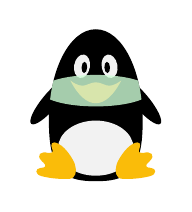
\begin{tikzpicture}
\penguin
\begin{scope}
  \clip (0.595, 0.92) .. controls (0.595, 0.26) and (0.355, 0.18) .. (0, 0.18) .. controls (-0.355, 0.18) and (-0.595, 0.26) .. (-0.595, 0.92) .. controls (-0.605, 1.58) and (-0.335, 2.11) .. (0, 2.11) .. controls (0.335, 2.11) and (0.605, 1.58) .. (0.595, 0.92) -- cycle;
%	\clip	(0.595, 0.92) .. controls (0.595, 0.26) and (0.355, 0.18) .. (0, 0.18) .. controls (-0.355, 0.18) and (-0.595, 0.26) .. (-0.595, 0.92) .. controls (-0.605, 1.58) and (-0.335, 2.11) .. (0, 2.11) .. controls (0.335, 2.11) and (0.605, 1.58) .. (0.595, 0.92) -- cycle;
%

  %\fill[blue,opacity=0.8](-4,1.2) ellipse (4,1.4);
  \fill[xkcdMint!50!white,opacity=0.8](0,1.33) ellipse [x radius=0.7, y radius=0.20];
\end{scope}
\end{tikzpicture}
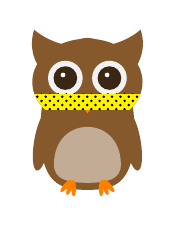
\begin{tikzpicture}
\owl
\begin{scope}
  \clip (0,1.55) ellipse[x radius=0.7, y radius=0.55];
%	\clip	(0.595, 0.92) .. controls (0.595, 0.26) and (0.355, 0.18) .. (0, 0.18) .. controls (-0.355, 0.18) and (-0.595, 0.26) .. (-0.595, 0.92) .. controls (-0.605, 1.58) and (-0.335, 2.11) .. (0, 2.11) .. controls (0.335, 2.11) and (0.605, 1.58) .. (0.595, 0.92) -- cycle;
%

  \fill[yellow](-4,1.2) rectangle (4,1.4);
  \fill[pattern=crosshatch dots](-4,1.2) rectangle (4,1.4);
\end{scope}
\end{tikzpicture}
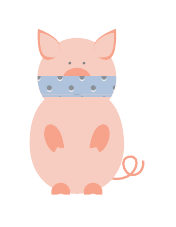
\begin{tikzpicture}
\pig
\begin{scope}
	\clip	(0,1.64) ellipse[x radius=.5, y radius=.5];

  \fill[pattern color=xkcdArmyGreen,pattern=crosshatch dots light steel blue](-3,1.4) rectangle (3,1.65);
\end{scope}
\end{tikzpicture}
%
%
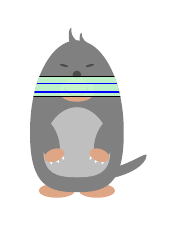
\begin{tikzpicture}
\moles
\begin{scope}
	\clip	(0.595, 0.92) .. controls (0.595, 0.26) and (0.355, 0.18) .. (0, 0.18) .. controls (-0.355, 0.18) and (-0.595, 0.26) .. (-0.595, 0.92) .. controls (-0.605, 1.58) and (-0.335, 2.11) .. (0, 2.11) .. controls (0.335, 2.11) and (0.605, 1.58) .. (0.595, 0.92) -- cycle;

  \fill[xkcdMint!60!white,opacity=0.9] (-3,1.4) rectangle (3,1.65);
  \draw[pattern color=blue,pattern=horizontal lines](-3,1.4) rectangle (3,1.65);
\end{scope}
\end{tikzpicture}
%
%
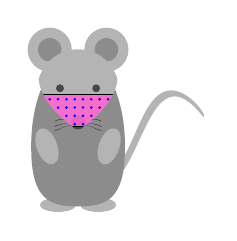
\begin{tikzpicture}
\mouse
\begin{scope}
	\clip	(0.5, 1.8) .. controls (0.5, 1.58) and (0.2, 1.25) .. (0, 1.16) .. controls (-0.2, 1.25) and (-0.5, 1.58) .. (-0.5, 1.8) .. controls (-0.34, 2.3) and (0.34, 2.3) .. (0.5, 1.8) -- cycle;

       \fill[xkcdBrightPink!60!white,opacity=0.9] (-3,1.2) rectangle (3,1.6);
       \draw[pattern color=blue,pattern=dots](-3,1.2) rectangle (3,1.6);
\end{scope}
\end{tikzpicture}
%%
%%

\begin{tikzpicture}
\panda
\begin{scope}
		\clip   (0.4897, 1.5886) .. controls (0.4614, 1.8238) and (0.25, 2.1172) .. (0, 2.1134) .. controls (-0.25, 2.1172) and (-0.4614, 1.8238) .. (-0.4897, 1.5886) .. controls (-0.5261, 1.3269) and (-0.2748, 1.2377) .. (0, 1.2377) .. controls (0.2748, 1.2377) and (0.5261, 1.3269) .. (0.4897, 1.5886) -- cycle;

       \fill[brown!60!white,opacity=0.8] (-3,1.4) rectangle (3,1.6);
\end{scope}
\end{tikzpicture}

\begin{tikzpicture}
\marmot
\begin{scope}
		\clip   (0.595, 0.92) .. controls (0.595, 0.26) and (0.355, 0.18) .. (0, 0.18) .. controls (-0.355, 0.18) and (-0.595, 0.26) .. (-0.595, 0.92) .. controls (-0.605, 1.58) and (-0.335, 2.11) .. (0, 2.11) .. controls (0.335, 2.11) and (0.605, 1.58) .. (0.595, 0.92) -- cycle;

       \fill[blue!20!cyan!30!white,opacity=0.8] (-3,1.3) rectangle (3,1.6);
\end{scope}
\end{tikzpicture}
%
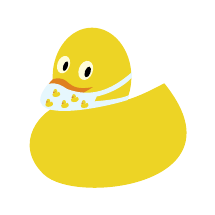
\begin{tikzpicture}
	\duck[]

  \begin{pgfinterruptboundingbox}
    \fill[cyan!10!white]  (1.4051,1.5586) .. controls (1.1370,1.3225) and (0.8775,1.2365) .. (0.5844,1.3462) .. controls (0.5190,1.3848) and (0.4601,1.4391) .. (0.3414,1.4100) .. controls (-0.1044,0.8610) and (1.0760,1.1140) .. (1.3547,1.2073) -- (1.3698,1.2679) .. controls (1.2783,1.2261) and (1.1035,1.2035) .. (0.9324,1.1895) -- (0.9600,1.2509) .. controls (1.1068,1.2809) and (1.2985,1.3700) .. (1.4071,1.4930) -- cycle;
  \end{pgfinterruptboundingbox}

  \duck[scale=0.05, shift={(6,22.3)}]
  \duck[scale=0.05, shift={(7.8,24.8)}]
  \duck[scale=0.05, shift={(10,22)}]
  \duck[scale=0.05, shift={(12.5,23.5)}]
  \duck[scale=0.05, shift={(15,22)}]

\end{tikzpicture}	
%
%
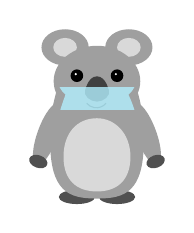
\begin{tikzpicture}
\koala
\begin{scope}
		\clip   (-0.1,2.1) to[out=180,in=140,looseness=1.2] (-0.4,1.5) to[out=-110,in=180,looseness=1.2] (-0.1,0.15) to[out=00,in=-65,looseness=1.2] (0.4,1.5) to[out=40,in=0,looseness=1.2] cycle;

       \fill[blue!20!cyan!30!white,opacity=0.8] (-3,1.3) rectangle (3,1.6);
\end{scope}
\end{tikzpicture}
%\begin{tikzpicture}
%\anteater
%%\begin{scope}
%%		\clip (0, 1.55) ellipse[x radius=0.42, y radius=0.2];
%%       \fill[mask!80!red] (-3,1.45) rectangle (3,1.65);
%%\end{scope}
%\end{tikzpicture}
%
%\begin{tikzpicture}
%\coati
%\begin{scope}
%		\clip   (0,2.1) to[out=180,in=140,looseness=1.2] (-0.3,1.5) to[out=-110,in=180,looseness=1.2] (0,0.15) to[out=00,in=-65,looseness=1.2] (0.3,1.5) to[out=40,in=0,looseness=1.2] cycle;
%
%       \fill[blue!20!cyan!30!white,opacity=0.8] (-3,1.5) rectangle (3,1.7);
%\end{scope}
%\end{tikzpicture}
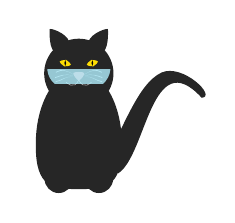
\begin{tikzpicture}
\cat
\begin{scope}
		\clip   (0,2.1) to[out=180,in=140,looseness=1.2] (-0.3,1.5) to[out=-110,in=180,looseness=1.2] (0,0.15) to[out=00,in=-65,looseness=1.2] (0.3,1.5) to[out=40,in=0,looseness=1.2] cycle;

       \fill[blue!20!cyan!30!white,opacity=0.8] (-3,1.5) rectangle (3,1.7);
\end{scope}
\end{tikzpicture}
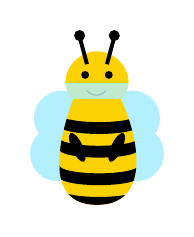
\begin{tikzpicture}
\bee
\begin{scope}
		\clip   (0,2.1) to[out=180,in=140,looseness=1.2] (-0.3,1.5) to[out=-110,in=180,looseness=1.2] (0,0.15) to[out=00,in=-65,looseness=1.2] (0.3,1.5) to[out=40,in=0,looseness=1.2] cycle;

       \fill[blue!20!cyan!30!white,opacity=0.8] (-3,1.5) rectangle (3,1.7);
\end{scope}
\end{tikzpicture}

\begin{tikzpicture}
\rhino
\begin{scope}
		\clip (0, 1.55) ellipse[x radius=0.42, y radius=0.2];
       \fill[mask!80!red] (-3,1.45) rectangle (3,1.65);
\end{scope}
\end{tikzpicture}

\begin{tikzpicture}
\hippo
\begin{scope}
		\clip (0, 1.55) ellipse[x radius=0.42, y radius=0.2];
       \fill[mask!80!red] (-3,1.45) rectangle (3,1.65);
\end{scope}
\end{tikzpicture}
\begin{tikzpicture}\bear\bearwear[shirt=white,t-shirt,body deco={\path (beartummy)--++(0.1,-0.1) pic[scale=0.04]{swisscross};}]
\begin{scope}
		\clip (0, 1.55) circle (0.5);
       \fill[mask!80!black] (-3,1.25) rectangle (3,1.6);
\end{scope}
\draw[\bear@body!70!white!80!red] (0, 1.5) ellipse (0.15 and 0.08);
\draw[\bear@body!30!black,line width=0.4pt] (0.145, 1.38) arc [start angle=-20, end angle=-160, radius=0.16];
%
%\path (0,0) pic{swisscross};
\end{tikzpicture}

\end{frame}
\end{document}